\begin{center}
\Huge
Opgaver i eksponentialregning
\end{center}
\stepcounter{section}

\subsection*{Opgave 1}

Aflæs fremskrivningsfaktoren og begyndelsesværdien for følgende eksponentialfunktioner.

\begin{align*}
	&a) \   f(x) = 2\cdot 1.03^x   &&b) \   f(x) = 7.64 \cdot 1.50^x \\
	&c) \   f(x) = 720 \cdot 3^x  &&d) \   f(x) = \sqrt{2} \cdot 0.5^x
\end{align*}


\subsection*{Opgave 2}

Bestem vækstraten for følgende eksponentialfunktioner
\begin{align*}
	&a) \ f(x) = 10\cdot 1.1^x  &&b) \ f(x) = 5\cdot  0.7^x
\end{align*}


\subsection*{Opgave 3}
En eksponentialfunktion $f$ er givet ved
\begin{align*}
	f(x) = 6 \cdot 2^x.
\end{align*}

\begin{enumerate}[label=\roman*)]
	\item Bestem $f(2)$.
	\item Bestem $f(6)$.
	\item Løs ligningen $f(x) = 96$.
\end{enumerate}

\subsection*{Opgave 4}

\begin{enumerate}[label=\roman*)]
	\item Udfyld følgende tabel og opskriv derefter forskriften for eksponentialfunktionen $f$.
	\item Undersøg, om du har udfyldt tabellen korrekt ved at bestemme $f(10)$. 
	\item Brug tabellen til at løse ligningen $f(x) = 15.76$.
\end{enumerate}

\begin{center}
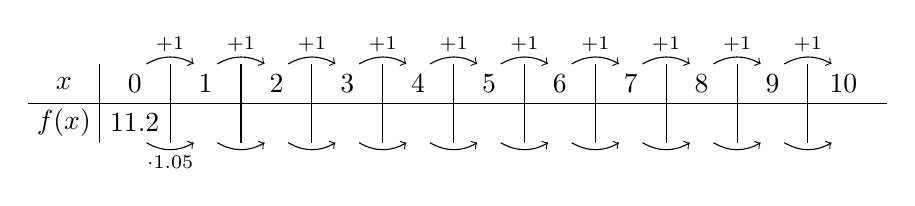
\begin{tikzpicture}
\foreach \i in {0,...,10}{
\draw (\i*0.9,0) -- (\i*0.9,1);
}
\draw (-0.9,0.5) -- (10,0.5);
\foreach \i in {0,...,10}{
\node at (\i*0.9+ 0.45,0.75) {$\i$};
}
\node at (0.45,0.25) {$11.2$};
\node at (-0.45,0.75) {$x$};
\node at (-0.45,0.25) {$f(x)$};
\foreach \i in {0,...,9}{
\draw [->] (\i*0.9+0.6,1) to [out=30,in=150] (\i*0.9+1.2,1);
\node at (\i*0.9+0.9,1.25) {$\scriptstyle+1$};
\draw [->] (\i*0.9+0.6,-0) to [out=-30,in=-150] (\i*0.9+1.2,-0);
}
\node at (0.9,-0.25) {$\scriptstyle\cdot 1.05$};
\end{tikzpicture}
\end{center}


\subsection*{Opgave 5}
En eksponentialfunktion $f$ går gennem punkterne $(2,8)$ og $(4,24)$.
\begin{enumerate}[label=\roman*)]
	\item Bestem forskriften for $f$.
	\item Bestem $f(5)$
\end{enumerate}

\subsection*{Opgave 6}
På planeten Flarp har beboerne fået sygdommen glub. Antallet af smittede på Flarp kan findes i \href{https://github.com/ChristianJLex/TeachingNotes/raw/master/2023-2024/Data%20og%20lign/smittede.xlsx}{\color{blue!60} dette datasæt}.

\begin{enumerate}[label=\roman*)]
	\item Lav eksponentiel regression på datasættet.
	\item Hvor mange glub-smittede er der efter 100 dage i følge modellen
\end{enumerate}
På Flarp bor 100 mio. flarpere. 
\begin{enumerate}[label=\roman*)]
	\setcounter{enumi}{2}
	\item Hvornår vil halvdelen af beboerne på Flarp være smittede med glub?
\end{enumerate}
